
\section{Durchführung der Trainingsläufe}

Im Laufe dieser wissenschaftlichen Arbeit werden eine Vielzahl an Trainingsläufen
durchgeführt. Die erfolgreichsten Agenten sind in Tabelle \ref{tab:TrainingRuns} zu sehen.
Außerdem stehen die Modelle und Videos des beobachteten Fahrverhaltens im Appendix zur
Verfügung. Im Folgenden werden die Versuche beschrieben und die vorgenommenen Adaptionen
an den Trainingsbedingungen begründet. Experiment 01 bezieht sich auf den Ansatz
der ursprünglichen Umsetzung von \emph{RobotSF} wie in \cite{machines11020268} und
dient als Grundlinie. Alle weiteren Experimente verwenden die Trainingsumgebungen
aus Abschnitt \ref{sec:TrainingApproach}.\\

\begin{table}[h]
  \centering
\begin{tabular}{ |p{1.5cm}||c|c|c|c|c|c|c|c| }
 \hline
 Training & Karte & Reward & Verkehr & Kinematik & Aktionen & $\Delta t$ & FE & PRF \\
 \hline \hline
 Exp. 01 & orig. & komplex & mittel    & Diff. Drive & wenig & 1 & nein & ja   \\ \hline
 Exp. 02 & klein & einfach & wenig     & Diff. Drive & wenig & 1 & nein & nein \\ \hline
 Exp. 03 & klein & einfach & viel      & Diff. Drive & wenig & 1 & nein & nein \\ \hline
 Exp. 04 & klein & einfach & viel      & Diff. Drive & wenig & 1 & nein & ja   \\ \hline
 Exp. 05 & klein & einfach & sehr viel & Diff. Drive & wenig & 1 & nein & ja   \\ \hline
 Exp. 06 & groß  & einfach & mittel    & Bicycle     & viel  & 3 & ja   & ja   \\ \hline
 Exp. 07 & groß  & einfach & mittel    & Bicycle     & viel  & 3 & ja   & ja   \\ \hline
 Exp. 08 & groß  & einfach & mittel    & Bicycle     & viel  & 3 & ja   & ja   \\
 \hline
\end{tabular}
\caption{Auflistung der Experimente und verwendeter Parameter}
\label{tab:TrainingRuns}
\end{table}

Zunächst liegt der Fokus bis einschließlich Experiment 05 auf einem Fahrzeug mit
Differential Drive Kinematik. Das Kartenmaterial besteht aus einigen miteinander verbundenen
Häuserblocks nahe des Universitätsgeländes, in deren Innenhöfen künstliche Fußgängerzonen
angelegt werden, um belebte Plätze zu simulieren. Das Fahrzeug startet in der Mitte
der Karte und folgt Routen in alle Himmelsrichtungen, die bewusst durch mindestens
eine Menschenmenge verlaufen. Durch die Wahl eines Zielradius von 1 Meter wird erzwungen,
dass der Fahragent lernt, sicher in die Menschenmenge einzutauchen und wieder herauszufahren.
Die \emph{Ped-Robot Force} (PRF) ist hierbei zunächst deaktiviert, sodass die Fußgänger
das Fahrzeug nicht wahrnehmen und demnach auch nicht ihrerseits ausweichen können.
Zudem liefert der LiDAR-Sensor nur die Entfernungen eines Zeitschritts (Standbild),
woraus für den Agent keine Fußgängerdynamiken ableitbar sind.
Des weiteren verfügt das Neuronale Netz des Agenten über keinen Feature Extractor (FE),
sondern verarbeitet flache, konkatenierte Feature-Vektoren aller Sensoren.
Die Fußgängerdichte wird während des Trainings auf 0.01 Fußgänger pro $m^2$
eingestellt, was einer relativ lückenhaften Menschenmenge entspricht und im Laufe der
Versuchsreihe hin zu moderaten Menschenmassen mit Dichte 0.04 erhöht. Anschließend
wird das Fahrverhalten der trainierten Agenten jeweils im Live Debugging begutachtet,
wobei schrittweise die Fußgängerdichte von 0.01 Fußgänger pro $m^2$ auf 0.08 angehoben wird.\\

Es kann bei den zugehörigen Experimenten 02 und 03 beobachtet werden, dass der Fahragent
erwartungsgemäß eine Strategie erlernt, die im fußgängerfreien Bereich geradlinig zum Ziel
fährt und beim Eintauchen in Menschenmengen ebenfalls zielstrebig eine Lücke findet,
um den jeweiligen Wegpunkt zu erreichen. Bei höheren Fußgängerdichten wird anstatt des
schnellen Eintauchens in die Menschenmenge ein abwartendes Verhalten beobachtet, wobei
der Agent so lange neben der Menge stehen bleibt, bis sich eine befahrbare Lücke öffnet.
Die gelernten Verhaltensweisen erfüllen zwar die von der Trainingsumgebung gestellte
Aufgabe, sind jedoch für praktische Erprobungen eher ungeeignet, da oftmals Situationen
vorliegen, bei denen kein Fortschritt zu erzielen ist, wenn nur außerhalb der
Menschenmenge gewartet wird.\\

Um praxistauglichere Verhaltensweisen zu erhalten, wird eine weitere Versuchsreihe
anhand der Experimente 04 und 05 mit moderaten bis hohen Fußgängerdichten und aktivierter
\emph{Ped-Robot Force} durchgeführt, sodass die Fußgänger nun das Fahrzeug sehen können
und eigenständig ausweichen. Die Kraft wird so gewichtet, dass ein stehendes Fahrzeug
relativ eng von den Fußgängern umlaufen wird. Dadurch muss der Agent keine Zusammenstöße
befürchten, ist aber zugleich zum Abwarten gezwungen, bis die Passage frei ist. Bei einem
entsprechend trainierten Agent wird ein Fahrverhalten beobachtet, bei dem das Fahrzeug
frontal in die Menschenmenge eintaucht und sich langsam je nach Freiraum vor dem
Fahrzeug vorwärts zum Wegpunkt bewegt. Wie in Abbildung \ref{fig:DiveIntoCrowd} zu
sehen ist, bleibt das Fahrzeug stehen und lässt die Fußgänger passieren, solange
es komplett von Fußgängern umgeben ist und wartet ab, bis erneut Fortschritte
zu erzielen sind. Diese Verhaltensweise liefert zufriedenstellende Ergebnisse,
jedoch lenkt der Agent nach dem Erreichen von Wegpunkten teilweise abrupt, da ihm
die Peilung des nächsten Wegpunkts nicht bekannt ist und er zudem durch eine niedrige
Aktionsfrequenz von nur 2.5 Aktionen pro Sekunde keine Möglichkeit für exaktere
Reaktionen hat.\\

\begin{figure}[h]
  \centering
  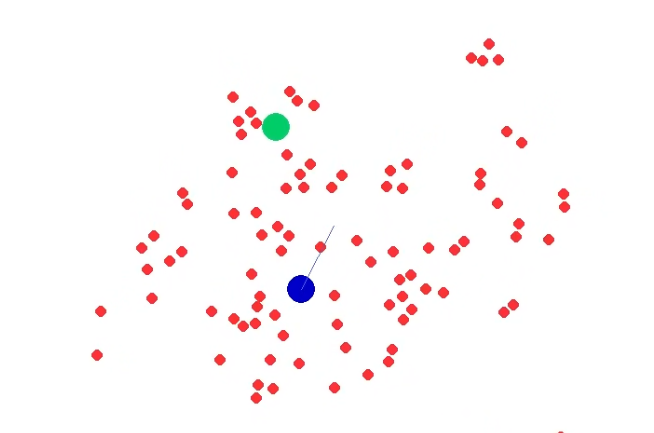
\includegraphics[width = 0.6\textwidth]{imgs/eintauchen_in_menschenmasse}
  \caption{Sicheres Durchqueren einer dichten Menschenmasse}
  \label{fig:DiveIntoCrowd}
\end{figure}

Um dynamischere Trajektorien fahren zu können, wird dem Agent eine zusätzliche
Zielpeilung des nächsten Wegpunkts bezüglich seiner aktuellen Orientierung
bereitgestellt. Zudem wird die Aktionsfrequenz auf 10 Aktionen pro Sekunde erhöht,
um eine exaktere Fahrweise zu ermöglichen. Der anschließende Trainingslauf bringt
jedoch keine wesentliche Verbesserung und wird deshalb verworfen. Es wird experimentell
nachgewiesen, dass die bei einer niedrigen Aktionsfrequenz trainierten Agenten in einer
Simulationsumgebung mit hoher Aktionsfrequenz gute Ergebnisse erzielen. Dies ist
vermutlich auf die sehr defensive Fahrweise der Agenten zurückzuführen, wofür nicht
so viele Aktionen pro Sekunde notwendig sind.\\

Da mit den bisherigen Trainingsläufen bereits sehr gute Verhaltensweisen in dichten
Menschenmengen erzielbar sind, wird nun eine größere Karte des Universitätscampus
als Trainingsumgebung verwendet, die Fußgängerrouten auf allen befahrenen Gehwegen und
einige Fußgängerzonen an Engstellen aufweist. Um die Erlernbarkeit der Steuerung eines
selbstfahrenden E-Scooters zu demonstrieren, wird eine zusätzliche Fahrzeugkinematik
anhand des Fahrradmodells erprobt. Zur Modellierung von Fußgängerdynamiken stehen
dem Agent die Sensordaten der letzten 3 Simulationsschritte zur Verfügung, welche mit
einem Feature Extractor vorverarbeitet werden.\\

Die aus den folgenden Experimente 06, 07 und 08 resultierenden Agenten sind durch die
neue Kinematik anhand des Fahrradmodells in der Lage, rückwärts zu fahren, wodurch
sich die erlernte Verhaltensweise stark ändert. Durch die zudem verbesserte Erkennung der
Fußgängerdynamiken können gefährlichere Fahrmanöver beobachtet werden, bei denen der
Agent auf einem Gehweg frontal auf einen entgegenkommenden Fußgänger zu fährt, im letzten
Moment stark rückwärts beschleunigt und dann eine ausweichende Kreisbahn einschlägt.
Eine entsprechende Verhaltensweise scheint für den echten Verkehr jedoch ungeeignet,
weshalb in der Fahrzeugkinematik das Rückwärtsfahren anschließend verboten wird.
Eine darauffolgende Auswertung ohne Rückwärtsfahren bestätigt die Annahme, dass der Agent
das Rückwärtsfahren aktiv in seinen Fahrmanövern einsetzt, da der Agent nun beim Ausweichen
rückwärts fahren möchte, aber nicht mehr kann und daraufhin mit dem Fußgänger kollidiert.\\

Weitere Experimente können aufgrund des beschränkten zeitlichen Rahmens dieser Arbeit
nicht mehr durchgeführt werden. Offene Fragen bleiben, wie gut ein Agent mit Differential
Drive Kinematik bzw. Fahrradmodell ohne Rückwärtsfahren in der großen Trainingsumgebung
des Universitätscampus lernt.
